\documentclass[a4paper,10pt]{article}
\usepackage[utf8x]{inputenc}
\usepackage[ngerman]{babel}
\usepackage{cite}
\usepackage{amsmath}
\usepackage{rotating}
\usepackage{graphicx}
\usepackage{epsfig}
\usepackage{hyperref}
\hypersetup{
%    bookmarks=true,
    pdftoolbar=true,
    pdfmenubar=true,
    pdffitwindow=false,
    pdfstartview={FitH},
    pdftitle={Die Pioneer-Anomalie},
    pdfauthor={Judith Selig, Michael F. Sch\"onitzer, Florian Schlagintweit},
    pdfsubject={Pioneer-Anomalie},
    pdfkeywords={Pioneer} {Anomalie} {Physik} {Raumfahrt},
    pdfnewwindow=true,
    colorlinks=true,
    linkcolor=black,
    citecolor=black,
    filecolor=black,
    urlcolor=blue
}

\usepackage[percent]{overpic}
\usepackage{color}
\usepackage{subfig}
\usepackage{placeins}


\newcommand{\rem}[1]{}

%opening
\title{Die Pioneer-Anomalie}
%\author{Judith Selig\footnote{judith.selig@gmx.de}, Michael F. Schönitzer\footnote{michael@schoenitzer.de}, Florian Schlagintweit\footnote{florian@schlagintweit.de}}	% welche Reihenfolge der Namen?
%\author{Judith Selig\thanks{judith.selig@gmx.de}, Michael F. Schönitzer\thanks{michael@schoenitzer.de}, Florian Schlagintweit\footnote{florian@schlagintweit.de}}	% welche Reihenfolge der Namen?

\author{Judith Selig\\judith.selig@gmx.de \and Michael F. Schönitzer\\michael@schoenitzer.de \and Florian Schlagintweit\\florian@schlagintweit.de}	% welche Reihenfolge der Namen?


\begin{document}

\maketitle

% \begin{abstract}

% \end{abstract}

\shorthandoff{"}

Im Februar 1969 genehmigte die NASA ( National Aeronautics and Space
Administration) ein Programm, um den Asteroidengürtel, das
interplanetare Medium zwischen Mars und Jupiter, die äußeren Planeten
und Fly-By Manöver zu erforschen. Hierzu wurden zwei baugleiche Sonden
Pioneer F (Pioneer 10 Mission) und Pioneer G (Pioneer 11 Mission) zum
Jupiter gebracht. Die Pioneer 10 Mission startete am 2. März 1972 und
wurde dann auf ca. 14,4 km/s beschleunigt. Die Sonde durchflog im Juli
1972 unbeschadet den Asteroidengürtel und erreichte am 4. Dezember 1973
den Jupiter. Hier nutzte man ein Fly-By Manöver um die Sonde auf eine
heliozentrische Fluchtgeschwindigkeit von 11,322 km/s
(Gesamtgeschwindigkeit 36,7 km/s)zu beschleunigen um das Sonnensystem
in Richtung des Sterns Aldebaran (Laut Zeitplan sollte die Sonde den
Stern in ungefähr 2 Millionen Jahren erreichen\cite{Nieto2007}) zu verlassen.
Pioneer 11 startete
13 Monate später, am 6. April 1973, da die NASA mit Pioneer 10 erst
herausfinden wollte, ob eine Durchquerung des Asteroidengürtels
überhaupt möglich ist. Ihre Bahn führte Pioneer 11 ebenfals Richtung
Jupiter, den sie am 2. Dezember 1974 erreichte. Das dort durchgeführte
Fly-By Manöver brachte sie auf eine Bahn, die Pioneer 11 zunächst
wieder innerhalb der Jupiter-Bahn führte, um dann aber am 1. September
1979 den Saturn zu erreichen (Abb. \$1) In einem weiteren Fly-By
Manöver, bei dem die Sonde die Ringe des Saturns unbeschadet durchquert
hat, wurde sie auf eine asymptotische Fluchtgeschwindigkeit von 10,450
km/s gebracht. Pioneer 11 steuert auf die Konstellation Aquila zu, wo
sie in ungefähr 4 Millionen Jahren eintreffen wird. Die Relationen der
Flugbahnen der Sonden Pioneer 10 und 11, sowie Voyager 1 und 2 sind in
Abb. \$2 zu erkennen.


\bigskip

Abb. \$1 und \$2

\bigskip

Obwohl Pioneer 10 und 11 nur auf eine Betriebszeit von 21 Monate
ausgelegt waren, sendete Pioneer 10 Messdaten bis zum 27. April 2002.
Das letzte Signal von Pioneer 10 erreichte die Erde am 23. Januar 2003.
Das letzte Signal von Pioneer 11 wurde jedoch deutlich früher, am 24.
November 1995 empfangen, da durch das zweite Fly-By Manöver am Saturn
sehr viel mehr Leistung benötigt wurde.
Zu den o.g. Missionszielen gehörte vor allem unter dem Punkte der
Erforschung der äußeren Planeten die Suche nach dem „Planeten X“, der
damals jenseits von Neptun vermutet wurde. Um das schwache
Gravitationsfeld dieses ominösen Planeten nachzuweisen und um möglichst
nahe an Jupiter und Saturn vorbei zu fliegen, benötigten die
Pioneer-Sonden eine sehr genaue Navigation. Dabei wurden von einer
Bodenstation des Deep Space Network DSN (in Goldstone/USA,
Madrid/Spanien, Canberra/Australien) Radiowellen mit einer
wohldefinierten Frequenz zur Sonde geschickt. Die Pioneers sendete
dieses Signal mit einer um den Faktor 240/221 konvertierten Frequenz
wieder zur Erde zurück\cite{Dittus2006}. Diese genaue
Navigation erlaubte schließlich die Entdeckung der Pioneer-Anomalie. 
Damit die Parabolantenne immer auf die Erde gerichtet blieb, musste
die Sonde vor allem nach Vorbeiflügen an großen Planeten neu
ausgerichtet werden. Hierzu wurden kleine Triebwerke für eine kurze
Zeit gezündet. Alle weiteren Störfaktoren auf die Flugbahn von Pioneer
10 und 11 wurden mit einer Eigenrotation der Sonden um die
Symmetrieachse der Parabolantenne von 4 bis 7 U/min
<<<<<<< HEAD
ausgeglichen\cite{Dittus2006}\cite{Nieto2007}.
Durch die genaue Navigation und die Verminderung von Fehlern,
bemerkte man Anfang der 80er eine unvorhergesehene Beschleunigung von
$(8,74+-1,33)*10^{-8} cm/s^{2}$ \cite{Anderson2002} in Richtung der Sonne. 
=======
ausgeglichen\cite{Dittus2006} \cite{Nieto2007}.
Durch die genaue Navigation und die Verminderung von Fehlern,
bemerkte man Anfang der 80er eine unvorhergesehene Beschleunigung von
$(8,74+-1,33)*10^{-8} cm/s^{2}$ \cite{Anderson2002}in Richtung der Sonne. 
>>>>>>> 7558b39e935f0730866b217868e1333178653123

Diese Beschleunigung wurde schließlich zur Pioneer-Anomalie, deren
Ursache bis heute nicht bekannt ist.


\section{Die Anomalie}

\subsection{Navigation und Geschwindigkeitsmessung}\label{messung}
Die Navigation der Pioneersonden erfolgte mithilfe der Antennen des Deep Space Network (DSN), einem Zusammenschluss mehrerer Radioteleskopanlagen des Jet Propulsion Laboratory (JPL)\footnote{Das Jet Propulsion Laboratory in Kalifornien entwickelt und steuert Sonden für die NASA und beschäftigt viele der Experten auf dem Gebiet der Pioneer-Anomalie, darunter auch John D. Anderson und Slava G. Turyshev.}. Das DSN besteht heute aus großen Radioteleskopanlagen in Goldstone/USA, Madrid/Spanien und Canberra/Australien. Früher gab es darüber hinaus noch Anlagen in Woomera/Australien und Johannesburg/Süd Afrika\cite{Anderson2002}\cite{Turyshev2010}. Dies sind jeweils Komplexe von zahlreichen Antennen – für die Navigation der Pioneer-Sonden wurden laut der Arbeit von Anderson et al.\cite{Anderson2002} davon die Deep Space Station (DSS) Antennen 12, 14, 42, 43, 62 und 63 verwendet. Turyshev und Toth erläutern jedoch in ihrer 2010 erschienenen Arbeit, dass noch etliche weitere Antennen auf alle Parks des DSN, sowie auch einige Antennen anderer Einrichtungen verwendet wurden.\cite{Turyshev2010} Die Antennen hatten Anfangs meist Durchmesser von 26 Metern, später häufig 34 oder 64 Meter, teilweise bis zu 70 Meter\cite{Turyshev2010}.
Man sollte erwähnen, dass diese Antennenkomplexe im Laufe der Zeit vielfach umgebaut wurden um den Anforderungen neuer Missionen gerecht zu werden. Dabei haben sich unter anderem auch die internen Frequenzen geändert\cite{Anderson2002}. Dies muss bei der genauen Betrachtung der Daten berücksichtigt werden, ist darüber hinaus jedoch auch eine Voraussetzung für die 30 Jahre lange Missionsdauer gewesen, da ansonsten die Reichweite der Antennen nur etwa 22 AU \footnote{Eine Astronomische Einheit (AE) oder englisch Astronomical Unit (AU) ist der Abstand zwischen Sonne und Erde $\approx$ 149,6 Millionen Kilometer.} betragen hätte.\cite{Turyshev2010}
Die Geschwindigkeitsmessung der Pioneersonden, welche für die Pioneer-Anomalie von zentraler Bedeutung ist, erfolgte über die Zwei-Wege-Dopplerverschiebung von Radiowellen.

\subsubsection{Entfernungs- und Geschwindigkeitsbestimmung }
Wir nehmen im folgenden an, dass die Sonde sich näherungsweise radial von uns wegbewegt – wir berechnen also genau genommen nur die Geschwindigkeit in Blickrichtung, dies muss bei den Analysen berücksichtigt werden.
Von den Bodenstationen wurden Radiowellen bekannter Frequenz (S-Band, $\sim$2,11 GHz) zum Satelliten gesendet (Uplink).
Die Frequenz wird mithilfe eines Wasserstoff-Masers erzeugt.
Damit werden äußerst präzise und stabile Referenz-Frequenzen von 5 MHz und 10 MHz erzeugt. Im Digital Controlled Oscillator (DCO), werden diese Frequenzen verwendet um mit Frequenzmultipliern ein Signal mit ungefähr 22 MHz zu erzeugten, welches dann mit dem Faktor 96 multipliziert wird um das zu sendende Signal von etwa 2,11 GHz zu erhalten. Nach einer Verstärkung wird das Signal mit einer der Antennen zum Raumsonde gesandt.\cite{Anderson2002}
Der Satellit empfängt das Signal dopplerverschoben:
\begin{equation}
\label{equ:doppler1}
 \nu_R = \frac{1}{\sqrt{1-\frac{v^2}{c^2}}}(1-\frac{v}{c})\nu_E
\end{equation}
Dabei ist $c$ die Lichtgeschwindigkeit, $v$ die Geschwindigkeit der Sonde und $\nu_E$ die Sendefrequenz des Signals auf der Erde und  $\nu_R$ die Frequenz des bei der Raumsonde ankommenden Signals.
Die Sonde antwortet unmittelbar mit einer 8-Watt Sendeanlage (Antennendurchmesser: 137 cm\cite{Markwardt2002}) und eines Transponders
mit einer um den festen (und exakten) Faktor $ \frac{240}{221} $ multiplizierten Frequenz:
\begin{equation}
\label{equ:Faktor}
\nu'_R = \nu_R\frac{240}{221} \approx 2,292 GHz
\end{equation}
Dies ist notwendig, da es sich bei den Radiosignalen um kohärente Wellen handelt und man so Verfälschungen durch Interferenz der hin- und rücklaufenden Wellen vermeidet\cite{Anderson2002}.
Beim Rückweg wird das Signal (Downlink) ein zweites mal identisch dopplerverschoben.
Das empfangene Signal ist also zweifach doppler- und um den Faktor $\frac{240}{221}$ verschoben.
\begin{equation}
 \nu'_E = \frac{1}{\sqrt{1-\frac{v^2}{c^2}}}(1-\frac{v}{c}) \cdot \frac{240}{211}\nu_R \, = \,
\frac{1}{1-\frac{v^2}{c^2}}(1-\frac{v}{c})^2 \cdot \frac{240}{211} \nu_E
\end{equation}
Die relative Verschiebung ergibt sich also zu
\begin{equation}\label{equ:rel}
 \frac{\nu'_E-\nu_E}{\nu_E} = \frac{\frac{19}{221}- \frac{461}{221}\frac{v}{c}}{1+\frac{v}{c}}.
\end{equation}
In einigen Quellen wird zur Veranschaulichung die konstante Frequenzverschiebung durch die Elektronik
vernachlässigt, was zur einfacheren Form führt:
\begin{equation}\label{equ:einf_rel}
 \frac{\nu'_E-\nu_E}{\nu_E} \approx -2\frac{v/c}{1+v/c} \approx -2 \frac{v}{c}
\end{equation}
Ist die Sendeantenne auch die Empfangsantenne, so spricht man von einer zwei-Wege-Messung, wenn Sender- und Empfängerantennen unterschiedlich sind, spricht man von einer drei-Wege-Messung\cite{Levy2009}. Bei den drei-Wege Doppler-Messungen besteht die Gefahr, dass ein unbekannter Zeitunterschied zwischen den Uhren der Antennen die Messung verfälscht. Daher verwendeten manche Analysen diese Daten nicht oder nur selten\cite{Anderson2002}, während andere sie mit zwei-Wege-Doppler-Daten gleich behandelten\cite{Markwardt2002}. Darüber hinaus gibt es eine Vielzahl an sogenannten Einwegs-Doppler-Messdaten, bei denen die Sonde von sich aus die Bodenstation kontaktiert hat. Da die Frequenz der Signalquelle im Weltraumfahrzeug nicht ausreichend genau bekannt ist, sind diese Daten für unsere Zwecke unbrauchbar und werden ignoriert. %schon oben, als footnote?

Unabhängig davon lässt sich die Entfernung $d$ der Sonde auch durch die Laufzeit $\Delta t$ des Signales bestimmen:
\begin{equation}
 2d = c \Delta t
\end{equation}
Dafür wird der Uplink per Phasenmodulation mit einem Signal versehen und das von der Sonde zurückgesendete Echo beobachtet. (Der Transponder der Sonde demoduliert und filtert es um es in den Downlink hinein zu modulieren.) Dieses Verfahren nennt man "ramping". % wirklich mit -ing?
Dabei muss man beachten, dass es durch das ständige Senden solcher modulierter Signale und die langen Laufzeiten zu Verwechselungen zwischen unterschiedlichen Signalen kommen kann. Dies muss von den Analyseprogrammen erkannt werden.

Somit hat man zwei voneinander unabhängige Messmethoden, was Konsistenzchecks,
Fehlerminimierung und dem Ausschluss einiger phänomenologischer Fehler ermöglicht. Nicht zuletzt kann man damit durch falsch gemessene Frequenzen verursachte falsche Dopplerdaten erkennen\cite{Anderson2002}.
Allerdings wurden die Laufzeitmessungen laut \cite{Anderson2002} nur bei der Analyse der Daten von Galileo und Ulysses (siehe unten), nicht bei den Pioneersonden verwendet. Von den Pioneersonden liegen Laufzeitmessdaten ("ramped-range") nur von der ersten Zeit der Mission vor. Im späteren Verlauf der Mission wurde diese Technik unbrauchbar, da die Bandbreite der Trägerfrequenz zu klein wurde um die modulierten Veränderungen zu detektieren\cite{Turyshev2010}. % "carrier tracking loop bandwidth"->"Bandbreite der Trägerfrequenz" richtig übersetzt? Erklären warum.

Aufgrund der Eigenrotation der Erde lässt sich außerdem aus der dadurch entstehenden Modulation der Doppler-Daten auch die 3-dimensionale Position der Sonde berechnen. Die Amplitude der Sinusförmigen Variation ist mit dem Deklinationswinkel und die Phase mit der Rektaszension verbunden. Die Position lässt sich dadurch aus einer, einige Tage langen, Reihe von Dopplerdaten bestimmen. Daraus kann man durch Berechnung der Dynamik der Raumsondenbewegung ebenfalls die Entfernung berechnen. Auch dies fließt in die Analysen mit ein.\cite{Anderson2002} % Wirklich die Phase?
%Aber nich besonders gut, wie wir später sehen werden!?	 	% mehr

%Laut Markward\cite{Markwardt2002} wurden die Effekte der Dopplerverschiebung auf dem Hinweg bereits beim Senden grob kompensiert, so dass die Frequenz des Signals, das die Sonde empfängt, bei etwa 2.11 GHz liegt.

Die Frequenzmessung erfolgte durch Zählen der Perioden und Vergleich mit einer Atomuhr\cite{Nieto2007}. %``Schwingungen'' als Formulierung überprüfen -  Perioden
Die Frequenz ist dabei einen Durchschnittswert, definiert über die Perioden in einem gewissem Zeitraum, Integrationszeitraum genannt. Die Integrationszeit lag zwischen 0.1 Sekunde und 100 Sekunden oder teilweise noch mehr\cite{Markwardt2002}.

%Zumindest im Zeitraum von 1987-1994 erfolgten die Messungen weitgehend regelmäßig, zusätzlich gab es zu einigen Zeitpunkten eine höhere Anzahl an Messungen\cite{Markwardt2002}. % sonst? ; später weniger?
Laut Markwardt\cite{Markwardt2002} erfolgten die Messungen weitgehend regelmäßig, es gab jedoch zusätzlich zu einigen Zeitpunkten eine höhere Anzahl an Messungen.

%Für die Navigation wurde daraus direkt die aktuelle Flugbahn berechnet, wir wollen uns jedoch im Folgendem auf den – für das Thema relevantere – 
% Vergleich der gemessenen Geschwindigkeit mit der berechneten Geschwindigkeit beschränken. % Oder doch nicht?


\subsubsection{Archivierung der Messdaten}

Gespeichert wurden die Daten ursprünglich im "Intermediate Data Record"-Format (IDR), nach einer Konversion dann im "Archival Tracking Data File"-Format (ATDF) auf Magnetbändern. Diese enthalten alle vom DSN gemessenen Daten, inklusive Signalstärke, Antennenausrichtung, Frequenz, Entfernung und Störungen\cite{Turyshev2010}. % range und residuals besser übersetzen.
Viele der ATDF Dateien wurden als Magnetbänder an das NSSDC-Archiv zur Archivierung gesandt, jedoch nicht alle – dazu mehr in Kapitel \ref{daten}\cite{Markwardt2002}.
Die Radio Metric Data Conditioning group (RMDC) von JPL's Navigations- und Missionsentwurfs-Abteilung las diese aus und konvertierte sie mit der Software STRIPPER in das Format "Orbit Determination File" (ODF\footnote{Nicht zu verwechseln mit dem verbreiteten Officeformat ODF.} oder ODFILE).
Darin enthalten sind\cite{Levy2008}:
\begin{itemize}
\item Die durchschnittliche Dopplerdrift über eine gewisse Zeitspanne – "Compression time" genannt
\item Die Dauer dieser Zeitspanne
\item Der Zeitpunkt in der Mitte des Intervalls\footnote{Was dem Zeitpunkt entspricht, als die Raumsonde das Signal empfing\cite{Levy2008}}
\item Die Sendefrequenz
\item Angaben dazu, welche DSN-Antennen das Signal geschickt und welche es empfangen haben
\end{itemize}
Auch die Laufzeitmessungen sind in den ODF-Dateien enthalten\cite{Anderson2002}.
Die Compression time beträgt in der Regel 10 s, 60 s, 600 s oder 1980 s\cite{Anderson2002}. % Stimmt das?

Die ODF-Dateien sind das eigentliche Werkzeug mit welchem die meisten an der Pioneer-Anomalie forschenden Teams arbeiten. Diese verwenden die ODF Dateien dann entweder direkt, oder wandeln sie in das Format ihrer Software um (im Fall von \cite{Anderson2002} ist das das NAVIO-Format).

Die Aufzeichnung der Messungen wurde leider nicht so sorgfältig und gründ\-lich durchgeführt, wie man es heute für die Analysen gerne hätte, da man die Anomalie ursprünglich für eine "Kuriosität" hielt\cite{Nieto2005}.
Die Rohdaten wurden von unterschiedlichen Analysten ausgelesen und das oben angesprochene Programm STRIPPER sollte die damals relevanten Navigationsdaten extrahieren\cite{Nieto2005}, wodurch Daten verloren gingen. % merge mit obigen Abschnitt? überprüfen
Dabei verwendeten die unterschiedlichen Analysten unterschiedliche Modelle und Datenbearbeitungsstrategien\cite{Nieto2005}.
Darüber hinaus wurden die Navigations-Daten nicht sorgfältig archiviert\cite{Nieto2005}.
Die Auswirkungen davon werden wir in Kapitel \ref{daten} noch diskutieren.


\subsubsection{Weitere Einflüsse auf die Messung}
Für die genauere Bestimmung der Bahn muss man einige Einflüsse auf die Messung berücksichtigen, welche wir im Folgenden erläutern wollen.

Da das Radiosignal zirkular polarisiert ist, muss bei der Berechnung die Rotation der Sonde berücksichtigt werden: Beim "Reflektieren" des Signals an der Antenne des sich drehenden Raumfahrzeugs kommt es zu einer von der Rotationsgeschwindigkeit abhängigen zusätzlichen Dopplerverschiebung. Jede Umdrehung der Sonde führt zu einer zusätzlichen Schwingung im Up- und im Downlink. Mit dem Frequenzverhältnis von Up- und Downlink ergeben sich insgesamt $(1+240/221)$ Schwingungen pro Umdrehung der Sonde\cite{Anderson2002}. %Ist "Schwingungen" das richtige Wort dafür
Gleichung \ref{equ:Faktor} muss wie folgt erweitert werden:
\begin{equation}
\nu'_R = \frac{240}{221}\nu_R - \eta\nu_{Spin} \quad \mathrm{mit}  \quad \eta = 1+ \frac{240}{221}\ .
\end{equation}
Die durchschnittliche Rotationsgeschwindigkeit liegt bei etwa 4,4 Umdrehungen pro Minute (rpm) für Pioneer 10 und etwa 7,25 rpm für Pioneer 11 und sank mit der Zeit\cite{Anderson2002}.
Hochqualitative Daten zum Eigenrotation (Spin) sind für Pioneer 10 nur bis zum 17. Juli 1990 verfügbar, als das DSN aufhörte Spinkalibrationen durchzuführen. Für spätere Daten muss der Spin des Raumschiffes durch Interpolation der Datenpunkte und den Daten des Imaging Photo Polarimeter (IPP) berechnet werden. Nach einem Manöver am 6. Juli 1993 reichte die Energie jedoch für dessen Betrieb nicht mehr aus. Analysten konnten jedoch noch etwa alle 6 Monate eine grobe Abschätzung des Spins aus Informationen der sogenannten ConScan-Manöver erhalten. % Conscan erklären
Bei ConScan – Kurzform für conical scan, auf deutsch auch Minimumpeilung – wird die Empfangsantenne kreisförmig bewegt und gemessen, wo das Signal am stärksten ist. Führt man dieses Verfahren mehrfach durch, kann man die ideale Ausrichtung der Antenne herausfinden. In Kombination mit einem Ausrichtungsmanöver des Raumfahrzeugs kann man damit auch die ideale Ausrichtung der Antenne der Sonde bestimmen.\cite{Anderson2002}
%aus Anderson2002:
%Conscan stands for conical scan. The receiving antenna
%is moved in circles of angular size corresponding to one
%half of the beam-width of the incoming signal. This pro-
%cedure, possibly iterated, allows the correct pointing di-
%rection of the antenna to be found. When coupled with
%a maneuver, it can also be used to find the correct point-
%ing direction for the spacecraft antenna. The precession
%maneuvers can be open-loop, for orientation towards or
%away from Earth-pointing, or closed-loop, for homing on
%the uplink radio-frequency transmission from the Earth.
Für die Daten nach 1995 wurde der Spin nicht mehr berechnet, auch wenn dies weiterhin mit den Aufgezeichneten ConScan-Daten möglich wäre. Außerdem ist die Spinachse nicht genau identisch mit der Phasenachse weshalb es eine sehr kleine, aber messbare, Sinusfunktion in den Dopplerdaten gibt. Daraus ließe sich ebenfalls die Spinrate für die nach 1993 gewonnen Daten berechnen – dies wurde bisher jedoch noch nicht gemacht.\footnote{Zumindest soweit uns bekannt.}
Die genaue Spinkalibrierung von Pioneer 11 ist aufgrund des Versagens eines Spin-down-Schubtriebwerks nicht möglich\cite{Anderson2002}.
Markwardt zeigte in seiner Analyse, dass für Pioneer 10 der Spin vernachlässigt oder durch den durchschnittlichen Spin von 4,4 rpm vereinfacht werden kann, ohne dass sich das Ergebnis nennenswert ändert\cite{Markwardt2002}.

Zu beachten ist, dass die Propagation des Signales vom Medium beeinflusst wird. Der Einfluss von interplanetarer Materie konnte durch einen Vergleich
der Daten mit denen der Cassini-Mission analysiert werden, da diese mehrere Frequenzbänder verwendete\cite{Dittus2006}. %mehr, richitg, quelle 
Der Einfluss der Ionosphäre und der Troposphäre auf das Singal wurde durch Implementation der International Reference Ionosphere (IRI)
beziehungsweiße der Global Mapping Functions (GMF) berücksichtigt\cite{Levy2008}. % Anderson auch?; ist das Propagation?; Erklären?

%Gerechnet wurde in der Standard-Epoche J2000.0. %mehr, wohin damit?

Die Bewegung der Sonde wurde in baryzentrischen Koordinaten gemäß ICRF beschrieben. % genauer
Da die gemessene Geschwindigkeit jedoch die Relativgeschwindigkeit zur auf der Erde stehenden Antenne ist,
muss man den Einfluss dieser Geschwindigkeit berechnen um die Geschwindigkeit und somit die Sondenbahn im baryzentrischen Koordinatensystem zu erhalten.
Anders gesagt enthält die Frequenzverschiebung noch einen weiteren Term bezüglich der Bewegung der Antenne. Aus Gleichung \ref{equ:doppler1} wird somit:
\footnote{Markwardt gibt in seiner entsprechenden Formel beide Male ein $c^2$ anstatt c an, wir vermuten dass es sich dabei nur um einen Tippfehler in der Arbeit handelt.}
\begin{equation}
\label{equ:doppler3}
 \nu_R = \frac{(1-\frac{v}{c})}{\sqrt{1-\frac{v^2}{c^2}}} \cdot \frac{\sqrt{1-\frac{v_E^2}{c^2}}}{(1-\frac{v_E}{c})} \cdot \nu_E 
\end{equation}
Zusammen mit den Effekten des Spins ergibt sich damit die gesamte Frequenzverschiebung in Abhängigkeit von der Sondengeschwindigkeit in baryzentrischen Koordinaten zu:
\begin{equation}
 \nu'_E = \left[ \frac{240}{221} \nu_E d_{\overline{ER}} - \eta \nu_{Spin} \right]  d_{\overline{RE}}
\end{equation}
Wobei $d_{\overline{ER}}$ und $d_{\overline{RE}}$ die Dopplerverschiebungsterme gemäß Gleichung \ref{equ:doppler3} sind.
Die Erde ist jedoch sehr dynamisch: um die Präzision, die für diese Belange gewünscht ist, zu erreichen, muss die Geschwindigkeit der Antennen auf der Erdoberfläche unter der Berücksichtigung von Prezission, Nutation,
siderischen Rotation, Polarbewegung, der Gezeitenkräfte und Platentektonischen Bewegungen bestimmt werden.
Die Angaben zu Abbremsung sowie Unregelmäßigkeit der Rotation, zur Polbewegung, die Love numbers\footnote{Von AEH Love beschriebene ``Proportionalitätsfaktoren zwischen den verschiedenen Verzerrungen sowie dem sich einstellenden Gravitationsfeld einer sphärisch symmetrischen, nichtrotierenden elastischen isotropen Kugel und einem äußerem an der Kugel angreifenden Grafitationsgradienten''\cite{Dittus2006}.} und der Chandler wobble\footnote{Spiralfomiges Schwingen
der Erdachse um 0,7 Bogensekunden mit einer Periode von 435 Tagen} % Begriffe (genauer) erklären?
wurden dabei direkt aus Messungen mit Lunar Laser Ranging (LLR)\footnote{Beim LLR wird die Laufzeit von am Mond von Spiegeln reflektierten Laserpulsen gemessen.},
Satellite Laser Ranging (SLR)\footnote{Beim SLR wird die Laufzeit von Laserpulsen zwischen einem Satellit und der Bodenstation gemesse.n} und Very Long Baseline Interferometry
(VLBI)\footnote{Dabei werden von zwei, interkontinental weit entfernten Radioteleskopen, die Signale inklusive
Zeitreferenz gespeichert und die Interferenz dieser Signale am Computer stimuliert.} bestimmt.
Diese Daten wurden früher von Publikationen der International Earth Rotation Service (IERS) und der United States Naval Observatory (USNO) zusammengetragen. Heute werden die Daten vom ICRF bereitgestellt,
zu welchen die Earth Orientation Parameters (EOP) des JPL viel beiträgt\cite{Anderson2002}.

Die Beobachtungen der Bodenstationen wurden mit Zeitangaben nach der Universal Time 1 (UT1)
\footnote{Durch astronomische Beobachtung gewonnene und um Einflüsse der Polschwankungen (mit Perioden über 7 Tage) korrigierte, mittlere Ortszeit des durch die Sternwarte von Greenwich führenden Nullmeridians}
parametrisiert gespeichert. Für die Analysen und
Berechnungen mussten diese Zeitangaben einerseits in die Internationale Atomzeit TAI, andererseits auch in die
Ephemeridenzeit umgerechnet werden. Auch hierfür verwendete man äußerst genaue Angaben zu Position, Geschwindigkeit und
Gravitationspotential der Antennen.\cite{Dittus2006} % stimmt das? Ander sagen as anderes...

An dieser Stelle sei erwähnt, das die beiden vorangegangenen Abschnitte sich primär auf die Berechnungen von Anderson et al. aus dem Jahr 2002 beziehen.
Wir werden im nächsten Kapitel sehen, dass es mehrere unabhängige Überprüfungen gegeben hat.
Diese verwenden zum Teil andere Koordinaten- und Zeitsysteme.
So rechnet das Programm ODESSEY mit der Barycentric Coordinate Time (TCB) im Barycentric Celestial Reference System (BCRS).
Dies spielt jedoch für die Betrachtung im Rahmen dieser Arbeit keine Rolle, da die Unterschiede gering sind und die meisten fortführenden Arbeiten auf die Berechnungen von Anderson et al. aufbauen.	%fortführende Arbeiten?

Man hat sogar einen möglichen Einfluss von mechanischer Deformation der Antennen der Bodenstationen durch ihr eigenes Gewicht,
Alterung, Wind, Tektonik, etc. abgeschätzt, und in die Fehlerrechnung mit einbezogen\cite{Dittus2006}. % mehr, Quelle (note: <10^-5 a_p)

% Es fehlt u.U. noch einige weitere Dinge die man hier erwähnen sollte

% (wo) kommt das rein:
% Da die im ODF format gespeicherten Messdaten nur die Zeit t2 (Signal an der Sonde) nicht jedoch
% die Zeitpunkte t1 (Sendezeitpunkt auf der Erde) und t3 (Empfangszeitpunkt auf der Erde) enthalten,
% müssen dise für die spätere Verwendung in Analysen durch Schritweiße Berechnung der
% "relativistic light time equations"" aus t2 errechnen.\cite{Levey2009} %FIXME: begriff übersetzen



\subsection{Theoretische Berechnungen}
Die ursprüngliche Navigationsberechnung erfolgte durch das Orbital Determination Program (ODP) des JPL.
Hierbei wird die Bahn im Rahmen des relativistischen Einstein-Infeld-Hoffmann-Modells (EIH Modell)
bis einschließlich zur Ordnung $(\frac{v}{c})^4$ berechnet.
Die Gravitation der Sonne, der neun Planeten und des Monds, wurden dabei als isotrope Punktmassen mit dem
PPN-Formalismus (parameterized post-Newtonian formalism) beschrieben\cite{Anderson2002}. Die Gravitation der größten
Asteroiden (ca. 0,2 Erdmassen) und Kometen wurden darüber hinaus gemäß des Newtonschen Gravitationsgesetz mit
ein berechnet.

%Auch die ``Terrestrial and lunar figure effects``,
%die Gezeiten der Erde und die physische Libration wurde mit berücksichtigt.
Die Propagation des Lichtes wurde relativistisch bis zu Ordnung $(\frac{v}{c})^2$ genau berechnet.
%Zu benutzen: Anderson 2002 + Physikjournal + Vorträge
Darüberhinaus wurden bei etlichen dieser Berechnungen eine Reihe von weiteren Einflüssen mit berücksichtigt, welche wir
weiter unten % unter klassische Erklärungen
erläutern werden.\footnote{An dieser Stelle werden oft auch die Einflüsse auf die Beobachtung genannt, welche wir jedoch
bereits im vorhergehenden Abschnitt besprochen haben.}

Natürlich kam schnell die Kritik auf, es könne sich bei der Anomalie um einen Fehler im ODP des JPL handeln.
Die erste Überprüfung erfolgte 1998 mit dem unabhängig entwickelten CHASMP/POEAS-Code des Aerospace
Corporation.
Eine zweite Bestätigung folge 2002 durch einen von C. Markward (Goddard Space Flight Center, GFSC) geschriebenen Code.
Eine weitere Bestätigung erfolgte 2006 durch den Orbit determination code HELIOSAT entwickelt von Ø. Olsen von der
Universität Oslo.
Im Jahr 2008 entwickelte die Groupe Anomalie Pioneer (GAP) eine eigene Software namens ODYSSEY,
mit welcher die Anomalie ebenfalls bestätigt werden konnte.

 
\begin{figure}[htbn]
\begin{center}
\noindent    
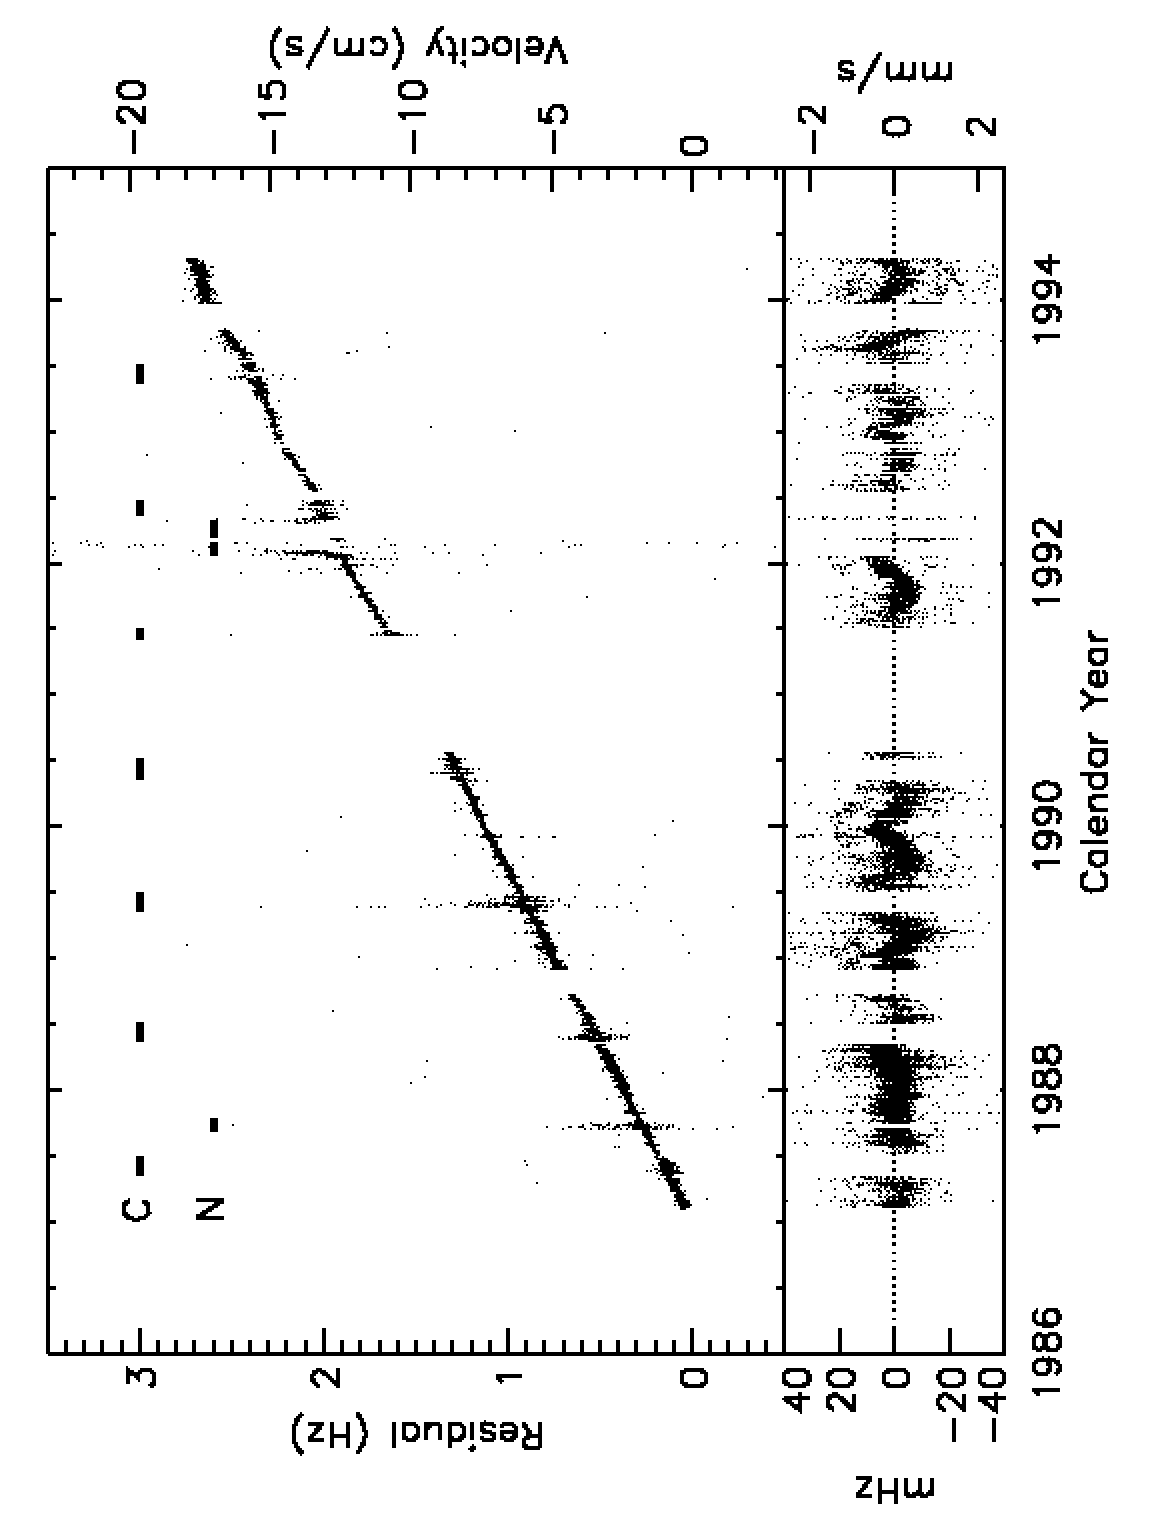
\includegraphics[angle=-90,width=0.8\linewidth]{images/M02P10beide}
\end{center}
\vskip -10pt
  \caption{Die Abweichungen von der Vorhergesagten Bahn. {\bf Oben:} ohne Berücksichtigung einer Anomalie; {\bf Unten:} mit Berücksichtigung der Anomalie. Die Beiden mit C und N markierten Zeilen oben, zeigen Zeiten an in welchen die Daten von der Auswertung ausgeschlossen wurden, weil die Daten durch Effekte Sonnen corona (C) beziehungsweise unbekannte Gründe (N) stark verrauscht waren. Es handelt bei diesem Bild um das Ergebnis von Markwardts Analyse\cite{Markwardt2002}.}\label{fig:Markwardvergl}
\end{figure} 
 
\begin{figure}[htnb]
\begin{center}
\noindent    
\psfig{figure=images/correlated,width=\linewidth,height=\textheight,keepaspectratio}
\end{center}
\vskip -10pt
  \caption{
Verlauf der anomalen Beschleunigung in Abhängigkeit von der Entfernung in Astronomischen Einheiten. Diese Tabelle zeigt das Resultat einer groben Auswertung der Daten an, sie ist noch kein Ergebnis der in Arbeit befindlichen, genauen Analyse der Daten über den gesamten Zeitraum. Die Ersterscheinung dieser Grafik konnte nicht ermittelt werden, sie taucht jedoch in zahlreichen Arbeiten auf, darunter\cite{Anderson2002}\cite{Nieto2005}\cite{Turyshev2010}
}
\label{fig:anomalie}
\end{figure} 
 
\subsection{Die Anomalie}
Geht man nun davon aus, dass unsere physikalischen Modelle richtig sind und wir alle relevanten Einflüsse berücksichtigt haben, so erwartet man im Rahmen der Messgenauigkeit für $a_P = 0$ eine Übereinstimmung im Fit.
Zunächst schien dies auch noch der Fall zu sein, nach dem Flyby-Manöver am Saturn im Jahr 1979 änderte sich dies für Pioneer 11 aber deutlich. Zu diesem Zeitpunkt befand sich die Sonde in einer Entfernung von etwa 20 AU und somit war die Beschleunigung durch den, in niedrigen Entfernungen nur ungenau berechenbaren, solaren Strahlungsdruck auf unter $5 \cdot 10^{-8} \frac{cm}{s^2}$ gesunken,
somit sank auch die Messungenauigkeit weit genug, um das nun zu Tage tretende Phänomen nicht mehr länger zu verschleiern.
Auch für Pioneer 10 stellte man bald darauf eine Abweichung fest.

Die Analyse der Daten von 1987 bis 1998 – das entspricht solaren Entfernungen von 20 bis 70 AU –
zeigte eine zeitlich konstant zunehmende anomale Blauverschiebung von
\begin{equation}
  \frac{d\Delta\nu}{dt}=(5,99\pm0,01)\cdot10^{-9}\frac{Hz}{s}
\end{equation}
wobei $\Delta\nu=[\nu_{Messung}-\nu_{Modell}]'_E$ ist\cite{Dittus2006}. Der Fehler hierbei ist nur der statistische Fehler. Die zunehmende Blauverschiebung ist im oberen Teil von Abbildung~\ref{fig:Markwardvergl} deutlich zu sehen. Lässt man die Software, die Bahn ohne eine Anomalie an die Werte fitten, so versucht sie  die Kurve durch Manöver anzupassen – man erhält dabei jedoch starke Abweichungen, weshalb ein solches Modell auszuschließen ist\cite{Markwardt2002}.

Lässt man, wie oben beschrieben, beim Fitten eine zusätzliche Beschleunigung zu, so erhält man eine wesentlich bessere Übereinstimmung (siehe Abbildung \ref{fig:Markwardvergl}, unten). Die dabei gefundenen Werte der Anomalie für die beiden Sonden sind:
\begin{eqnarray}
  a_{Pioneer 10} = (7,84\pm0,01)\cdot10^{-8}\frac{cm}{s^2} \\  
  a_{Pioneer 11} = (8,55\pm0,02)\cdot10^{-8}\frac{cm}{s^2}
\end{eqnarray}

Zwischen den obigen Werten lässt sich aus Gleichung (\ref{equ:rel}) ein direkter physikalischer Zusammenhang ableiten. Verwendet man die vereinfachte Version (\ref{equ:einf_rel}), so erhält man:
\begin{equation}
  a_{Pioneer}=\frac{dv}{dt}=\frac{1}{2}\frac{c}{\nu_E}\frac{d\Delta\nu}{dt}
\end{equation}
%oder
%\begin{equation}
%  \Delta\nu=-\nu_E \frac{2a_p t}{c}
%\end{equation}

Berücksichtigt man den Einfluss aller bekannter Effekte auf den Wert und die Unsicherheit der Größe\cite{Turyshev2004}, so erhält man einen endgültige Wert von:  
\begin{equation}
  a_{Pioneer} = (8,74\pm1,33)\cdot10^{-8}\frac{cm}{s^2}
\end{equation}

Andere Arbeiten mit den  unterschiedlichen Orbit Determination Codecs bestimmten die Beschleunigung zu $(7,70
\pm0,02)\cdot10^{-8}\frac{cm}{s^2}$ (Markwardt, 2002)\cite{Markwardt2002} beziehungsweise % anderen Wert von Markward
$(8,4\pm0,1)\cdot10^{-8}\frac{cm}{s^2}$ (Levy et al., 2008)\cite{Levy2008}.
Wobei beide Arbeiten sich nur auf Pioneer 10 beziehen und jeweils nur die statistischen Fehler angeben.
Wir wollen uns im folgenden jedoch – wie auch praktisch jede Arbeit der Fachliteratur – auf den oben angegebenen von
Anderson et al. berechneten Wert beschränken.
%% wohin damit:
% Die Standartabweichung bei einem Fit mit dieser konstanten Beschleunigung ist deutlich kleiner als ohne. % 9,8 mHz bei Levy

Der Wert mag zwar klein erscheinen, doch ist seine Größenordnung nur das $10^{-5}$ fache der Newtonschen Beschleunigung,
und er ist größer als die Faktoren $U/c^2$,$v^2/c^2$,$r a/c^2$ zur relativistischen Korrektur der newtonschen Dynamik.
% richtig?
Seit 1979 ist die Sonde um fast eine halbe Million Kilometer von der berechneten Bahn abgewichen:
\begin{equation}
  \Delta x= \frac12 \cdot a_p \cdot (2011-1979)^2 a^2\approx 445.000 km
\end{equation}

Diese Frequenzverschiebung wurde mit nur maximal 3\% Unterschied bei beiden Pioneer-Sonden unabhängig voneinander
gefunden. Das anomale Signal variiert über den analysierten Zeitraum um nur maximal 3,4\%\cite{Turyshev2004}.
Olsen zeigt jedoch, dass es bei der derzeitigen Datenlage nicht auszuschließen ist, dass die Anomalie mit der Zeit abnimmt.\cite{Olsen2006}
Die Richtung der
Beschleunigung ist mit einer Auflösung von 3° bisher noch recht ungenau bestimmt worden. Es ist daher nicht sicher möglich
zu sagen ob die Beschleunigung
in Richtung Sonne, Erde, negativer Geschwindigkeit oder Drehachse geht, dazu mehr in Kapitel \ref{fragen}.

Eine alternative Interpretation zu einer konstanten Beschleunigung, wäre eine zeitliche Beschleunigung.
So ließe sich die Anomalie auch durch eine zeitliche Beschleunigung von $a_t = (2,92 \pm 0,044) \cdot 10^{-18} s^{-2}$ schreiben.



\subsection{Variabler Teil}
Während in Normalfall die Anomalie als konstante Beschleunigung angesehen wird, wiesen betreits Anderson et al. in
ihrer Arbeit im Jahr 2002 darauf hin, dass es periodische Anteile in der Pioneeranomalie zu geben scheint. Im Jahr 2008
zeigte die „Groupe Anomalie Pioneer“ (GAP) – ein Zusammenschluss von etlichen französischen Forschungseinrichtungen –
das sich die Qualität des Fits nennenswert steigern lässt, wenn man zusätzlich zur konstanten Beschleunigung
periodische Terme verwendet.
Dabei ist es ihnen gelungen eine Beziehung zwischen dem Unterschied der Azimutalwinkel zwischen Sonde und Erde, sowie
den zeitlich veränderlichen Anteilen der Pioneeranomalie zu finden. %bäh

Die periodischen Anteile des Signals lassen sich sehr gut auf der auf Abb. FIXME dargestellten Spektralanalyse
erkennen. Die Drei großen Peaks liegen bei $f_1=0.9974\pm0.004\ Tagen$, $f_2=\frac12(0.9974\pm0.004)\ Tagen$ und 
$f_3=189\pm32\ Tagen$. Bedenkt man das 1.0 siderischer Tag = 0.9972 Tage ist, so entspricht dies genau
halbtägigen, täglichen und halbjährlichen Schwankungen. Anderson et al. ziehen dafür Messfehler – wie Fehler in den
Ephemeriden oder der Ausrichtung der Drehachse der Erde oder fehlerhafte Koordinaten der Messstationen – in Betracht.
Die Gruppe um Levey (GAP) hält dies jedoch für unwahrscheinlich, da diese Daten durch andere Beobachtungsmethoden
gestützt werden.
Sie nehmen an, dass durch eine beliebige Ursache die Ausbreitung des Tracking-Signals auf dem Weg zwischen Raumsonde und
Erde verändert wird. Sie beschreiben die Ursache als Funktion des Azimutalwinkel zwischen Sonde und Erde und fitten
dann die Fouriekoeffizienten. Dieses geometrische Modell beschreibt sowohl die täglichen, also auch die jährlichen
Schwankungen und verringert die Abweichung von den Messwerten von 9.8 mHz auf 5.5 mHz. Auch die Spektralanalyse (
Abb. FIXME) dieses fits zeigt die Verbesserung deutlich.

\bigskip
\bigskip

\section{Zukünftige Forschung}
\subsection{Neue Analyse aller Vorhandener Daten}
Die Analyse von Anderson et al., 2002 betrachtete nur die Pioneer 10-Daten in der Zeit vom 3. Januar 1987 bis zum 22.
July 1998 (40 AU bis 70,5 AU) und die Pioneer 11-Daten vom 5. Januar 1987 bis zum 1. Oktober 1990 (22,4 AU bis 31,7
AU). Jedoch empfing man bis zum 27. April 2002 brauchbare Daten von Pioneer 10. (Die Daten von Pioneer 11 waren ab
Oktober 1990 nicht mehr brauchbar) Auch die anderen erwähnten Analysen bezogen sich immer auf etwa den selben Zeitraum.

Die Daten von Pioneer 10 aus dem Zeitraum von 1998 bis 2002 wurden also noch nicht untersucht. Noch
Erfolgversprechender wäre jedoch eine Analyse der frühen Daten. Die Anomalie wurde bereits ab 1979 beobachtet und durch
bessere Berechnung des solaren Strahlungsdruck könnten auch die noch früheren Daten wichtige Informationen liefern. Ees
ist daher geplant die kompletten Daten, vom Start der Sonden, bis zu den letzten verwertbaren Signalen neu zu
analysieren.

% Es ist geplant am ZARM in Zusammenarbeit mit dem JPL die gesammten Pioneer Daten vom Start bis zum letzten Signal neu
% zu analysieren	% aus Physikjournal

% Wohin mit ``bei 20 AU (~1980) sinkt der solare Strahlungsdruck auf unter 5*10^-8 cm/s^2''?

\bigskip
…
\bigskip


\subsection{Die Bedeutung der Richtung der Anomalen Beschleunigung}
\bigskip
…
\bigskip


\bigskip
\section{Modifizierte Newtonsche Mechanik (MOND)}

Die modifizierte newtonsche Mechanik (MOND) wurde Mitte der 1980er Jahre
von Mordehai \ Milgrom als Gegenentwurf zur dunklen Materie entwickelt.
Ihre ursprüngliche Motivation ist es die gemessene abflachende
Rotationskurve von Galaxien zu erklären, die sich deutlich von der
Kurve unterscheidet, die nach den keplerschen Gesetzten berechnet
wurde. Das soll erreicht werden indem das zweite newtonsche Gesetz bzw.
das Gravitationsgesetz modifiziert wird. 


\bigskip

Das zweite newtonsche Axiom besagt, dass eine Masse m an der eine Kraft
F anliegt die Beschleunigung a erfährt: 

\begin{equation*}
F=m\cdot a
\end{equation*}
Dieser Zusammenhang kann allerdings für sehr kleine Beschleunigungen nur
sehr schwer bis gar nicht experimentell überprüft und nachgewiesen
werden. In Galaxien bewirkt die Schwerkraft der Sterne aber nur solche
kleinen Beschleunigungen, da sie sehr weit voneinander entfernt sind.
Milgroms Idee \cite{Bekenstein1984} war es daher das zweite newtonsche Gesetz für sehr
kleine Beschleunigungen abzuwandeln in

\begin{equation*}
F=m\cdot a\cdot \mu (a/a_{0})
\end{equation*}
 $a_{0}$ ist eine neue Naturkonstante, die angibt ab welchen
Beschleunigungen die Modifikation wirksam wird. Milgrom bestimmte sie
aus den Messungen der Rotationsgeschwindigkeiten möglichst vieler
Galaxien als ungefähr

\begin{equation*}
a_{0}=2\cdot 10^{-10}\frac{m}{s^{2}}
\end{equation*}
 $\mu (x)$ ist eine unspezifizierte Funktion welche folgende Bedingungen
erfüllt:

\begin{itemize}
\item  $\mu (x\gg 1)\approx 1$, so dass für große Beschleunigungen die
newtonsche Mechanik gilt
\item $\mu (x\ll 1)\approx x$
\end{itemize}
In der Literatur sind für  $\mu (x)$ am häufigsten verwendeten
Funktionen:

{\centering  $\mu (x)=\frac{x}{1+x}$ $\mu
(x)=\frac{x}{\sqrt{1+x^{2}}}$\par}

Will man jetzt MOND in Hinblick auf die Pioneer Anomalie \cite{Turyshev2010}
überprüfen, muss man als erstes betrachten, welche Auswirkungen die
Theorie auf die Zentripetalbeschleunigung  $a_{z}$ einer Masse m hat,
die sich im Gravitationsfeld eines Körpers der Masse M befindet.

Nach Newton gilt mit der Gravitationskonstante G:

{\centering  $F_{g}=\frac{G\cdot {M\cdot m}}{r^{2}}$\par}

Damit gilt für  $a_{z}$

\begin{equation*}
a_{z}=\frac{v^{2}}{r}=\frac{G\cdot {M}}{r^{2}}
\end{equation*}
Löst man diese Gleichung nach  $v^{2}$ auf, so erhält man:

\begin{equation*}
v^{2}=\frac{G\cdot M}{r}
\end{equation*}
Nach MOND gilt für sehr kleine Beschleunigungen:

\begin{equation*}
a_{z}\mu (\frac{a_{z}}{a_{0}})=\frac{G\cdot {M}}{r^{2}}
\end{equation*}
Da  $\frac{a_{z}}{a_{0}}\ll 1$ gilt  $\mu
(\frac{a_{z}}{a_{0}})=\frac{a_{z}}{a_{0}}$

Setzt man dies nun in die obige Gleichung ein und löst nach  $a_{z}$
auf, so erhält man:

\begin{equation*}
a_{z}=\frac{\sqrt{M\cdot G\cdot a_{0}}}{r}
\end{equation*}
Mit  $a_{z}=\frac{v^{2}}{r}$ erhält man hier für  $v^{2}$

\begin{equation*}
v^{2}=\sqrt{M\cdot G\cdot a_{0}}
\end{equation*}
Zusammenfassend gilt also nach der modifizierten newtonschen Dynamik:

\begin{itemize}
\item  $v^{2}=\frac{G\cdot M}{r}$ für  $a_{z}\gg a_{0}$ oder kleine
Abstände
\item  $v^{2}=\sqrt{M\cdot G\cdot a_{0}}$ für  $a_{z}\ll a_{0}$ oder
große Abstände
\end{itemize}
Betrachtet man nun die Pioneer Anomalie, kann man davon ausgehen, dass 
$a_{0}\ll \frac{G\cdot M}{r}$.

Wählt man nun  $\mu (x)=1+\frac{\zeta }{x}$ bekommt man für  $a_{z}$
folgendes Ergebnis:

\begin{equation*}
a_{z}=-\ \frac{G\cdot M}{r^{2}}-\zeta \cdot a_{0}
\end{equation*}
Für  $\zeta =7$ ist 

\begin{equation*}
\zeta \cdot a_{0}=8,4\cdot 10^{8}\frac{\mathit{cm}}{s^{2}}
\end{equation*}
was der anomalen Beschleunigung der Pioneer-Sonden entspricht.

% ToDo:
%% - Wohin mit ``bei 20 AU (~1980) sinkt der solare Strahlungsdruck auf unter 5*10^-8 cm/s^2''
%%     und allgemein der Beschreibung, Bedeutung und Berechnung des solaren Strahlungsdrucks?
%% - S-Band ist für 3-D wenig geeignet. (Route to Understanding)  -> ?
%% - Abgrenzung Navigation <> Einleitung
%% - ...

% ToFix:
%% - Quellen-format fixen
%% - Footnote der Authoren
%% - evtl. Anführungszeichen richten
%% - Namen im Text vereinheitlichen

\bibliography{lit}{}
\bibliographystyle{unsrtdin}

\end{document}
